\documentclass{scrartcl}
\usepackage{microtype}
\usepackage{amsmath}
\usepackage[english]{babel}
\usepackage{graphicx}

\begin{document}
    \section*{Tasks}
    \subsection*{1) Local measurement}
    The measurements for this section were run using graphs with 1000 nodes with density ranging from $1\%$ to $100\%$ of possible edges added. Note that overlaps aren't checked when adding edges to the graph, so a graph generated with $100\%$ of possible edges may not necessarily be a full graph.

    The charts below maps the dependency of time on graph density and path distance ($-1$ represents an unsuccessful search) . Time is measured in microseconds.
    \begin{center}
        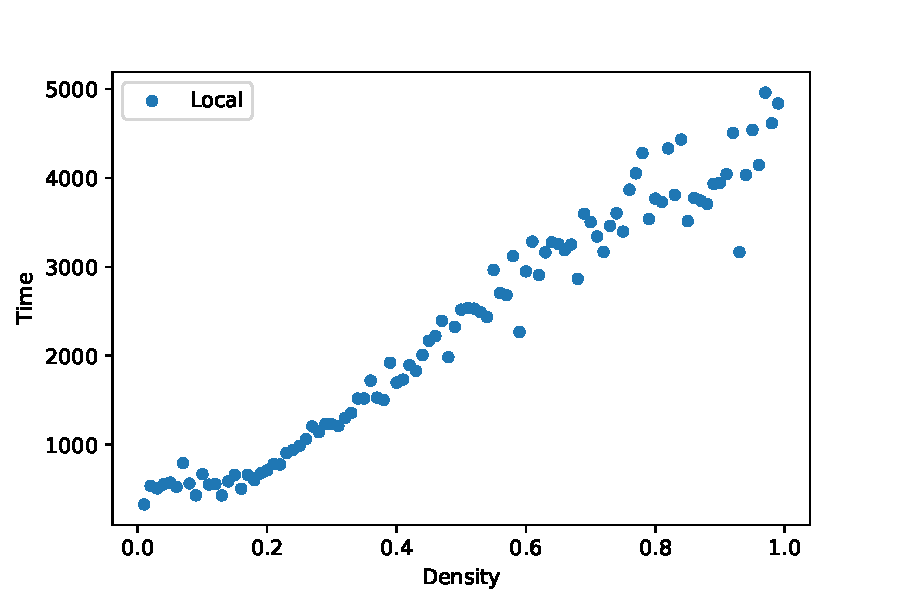
\includegraphics[width=0.8\linewidth]{picture.pdf}
        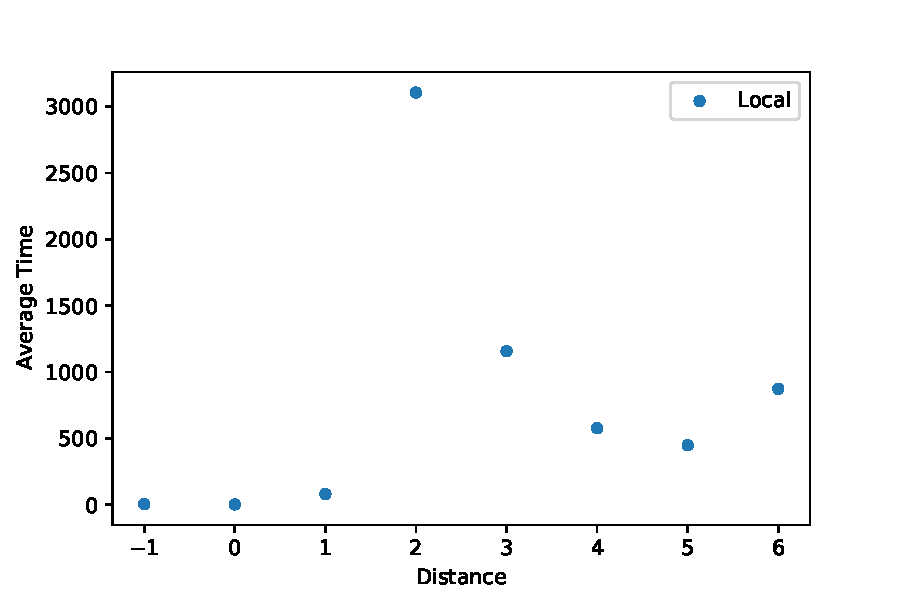
\includegraphics[width=0.8\linewidth]{picture_dist.pdf}
    \end{center}
    We can see that time increases linearly with density. This is expected, as more edges mean more possible paths to walk through and the BFS algorithm runs in $O(n+m)$ time.

    The distribution of average times based on distance is somewhat more surprising. One could reasonably expect the complexity to increase with distance, but that doesn't appear to be the case. We believe that the reason for this plot lies once again in the graph density. On dense graphs, shorter paths are more common, increasing their average time. Longer paths will be more common on sparse graphs, which take less time to enumerate.
    \subsection*{2) Remoter Searcher}
    \subsubsection*{Question} \
    The first time the remote serializer is passed a Node object as a parameter, That object needs to be serialized and sent over the network to the server. Because the node includes references to its neighbors, those also have to be serialized, as well as their neighbors and so on. The result is that all nodes reachable from the passed node are sent at once during the start of the search. The serializer then accesses those local copies during its search.

    \subsubsection*{Measurements}
    The measurements for this section were run using the same parameters as the previous task. On the charts below is a comparison between times spent searching with a local searcher vs. a remote one. Time is measured in microseconds.
    \begin{center}
        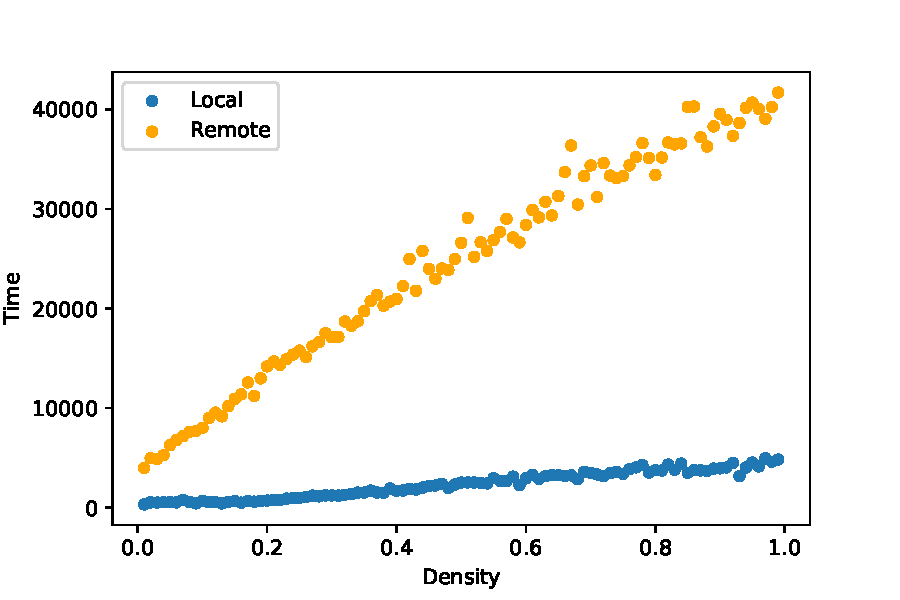
\includegraphics[width=0.8\linewidth]{picture2.pdf}
        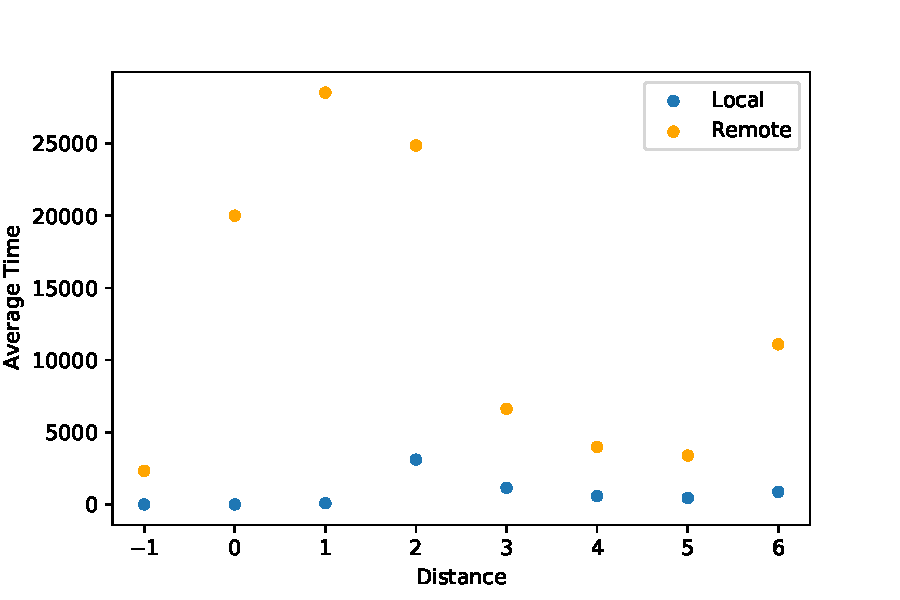
\includegraphics[width=0.8\linewidth]{picture_dist2.pdf}
    \end{center}
    The time complexity of a remote searcher also increases linearly, but its values are higher and its slope steeper. The difference can be attributed to the initial serialization. As the density of a graph increases, so does the amount of data that needs to be transferred over the network. This transfer then causes the observed delay. The relationship between distance and time exhibits the same behavior as in the local case, except of course with the added latency of network transfer.
    \subsection*{3) Remote Nodes}
    \subsubsection*{Question}
    When a remote factory creates a new node, it sends a stub to the local caller. When the local searcher then calls methods of that node, they are proxied to the remote instance. Accessing neighbors of a node then also returns the corresponding stubs. This means that there isn't a big serialized object sent at the beginning of the search, but every call to get neighbors of a node results in a separate network request.

    \subsubsection*{Measurements}
    See the following section.
    \subsection*{4) Remote Nodes and Searcher}
    \subsubsection*{Question}
    As in the previous task, the local process only receives stubs of the created nodes. When it then passes those nodes to the remote searcher, only a reference to those stubs is sent. The searcher then matches them with the corresponding remote object and all searching forward is done purely using server-side objects without any need for accessing client-side data. 

    \subsubsection*{Measurements}
    Measurements with remote nodes were done using graphs with 200 points due to their increased latency. Otherwise the methodology remains the same as in the first two tasks.
    \begin{center}
        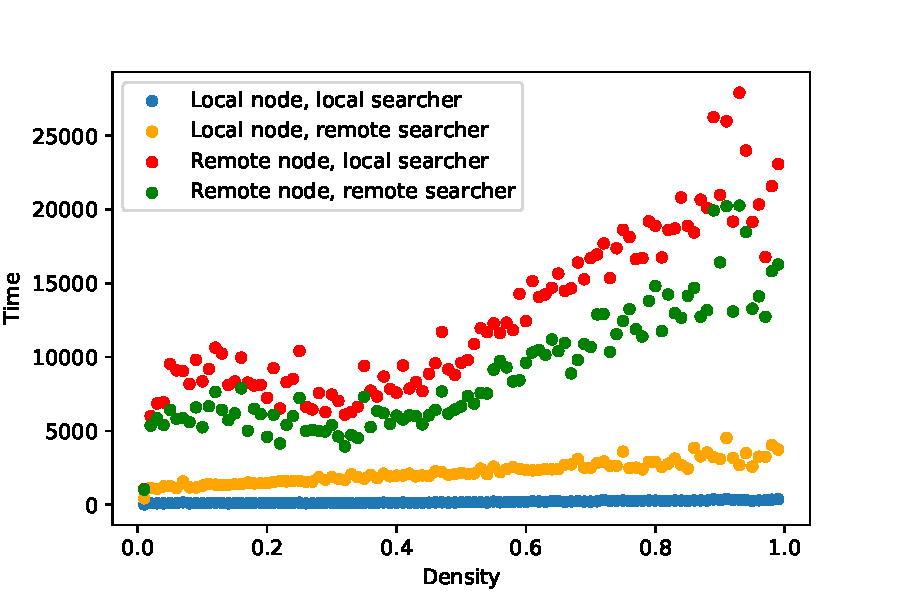
\includegraphics[width=0.8\linewidth]{picture34.pdf}
        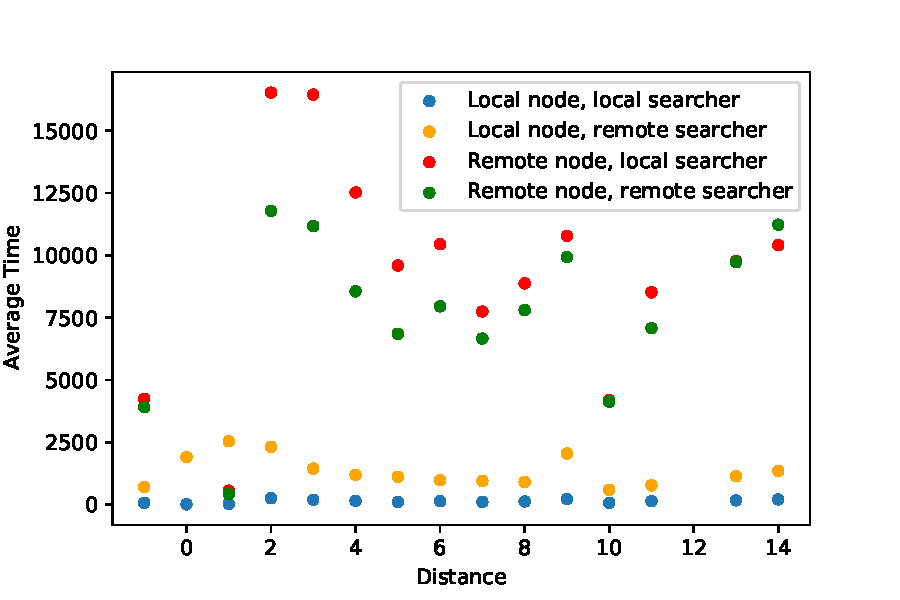
\includegraphics[width=0.8\linewidth]{picture34_dist.pdf}
    \end{center}
    From these charts we can see that computation with remote nodes is noticeably more time-consuming than computation with local nodes. This suggests that there is a lot more network communication happening in this mode compared to using local nodes. The variant with a remote searcher fares slightly better in comparison, but still lags significantly behind local node methods.


\end{document}